%=======================================================================
% 中文版前言 — RetNet-272M 技术报告
% 编译：xelatex 两遍（生成目录与交叉引用）
%=======================================================================
\documentclass[11pt,openany]{ctexart}

% =====================================================================
%  preamble-common.tex
%  Shared preamble for the RetNet-272M technical report (Chinese and
%  English editions).  Build with XeLaTeX.
%
%  Typographic convention (deliberately plain, single column, as in a
%  conventional technical report):
%    * serif body text, no coloured display headings
%    * numbered tables and figures, each with a caption
%    * remarks set as an indented, labelled passage rather than a
%      coloured box
% =====================================================================

\usepackage{amsmath}
\usepackage{amssymb}
\usepackage{bm}

% ---------- layout ---------------------------------------------------
\usepackage[a4paper,top=2.5cm,bottom=2.5cm,left=2.4cm,right=2.4cm]{geometry}
\usepackage{fancyhdr}
\usepackage{titlesec}
\usepackage{enumitem}
\usepackage{booktabs}
\usepackage{array}
\usepackage{tabularx}
% A table taller than a page must be able to break across pages: an unbreakable
% `tabular` that large is shipped out past the paper edge (Overfull \vbox), and
% the part below the edge is what the reader loses.  `longtable` is used only
% for such tables (see mktex.render_table).
\usepackage{longtable}
\usepackage{ragged2e}
\usepackage{xcolor}
\usepackage{caption}
\usepackage{graphicx}

% ---------- code -----------------------------------------------------
\usepackage{listings}
\usepackage{newunicodechar}

% ---------- references ----------------------------------------------
\usepackage[hidelinks,bookmarksnumbered]{hyperref}
\usepackage{bookmark}

% ---------- colours (used sparingly: code and rules only) ------------
\definecolor{codebg}{RGB}{248,248,249}
\definecolor{codeframe}{RGB}{216,220,225}
\definecolor{codecomment}{RGB}{104,124,108}
\definecolor{codekeyword}{RGB}{0,80,150}
\definecolor{codestring}{RGB}{160,60,40}
\definecolor{rulecol}{RGB}{178,182,188}
\definecolor{headrule}{RGB}{40,48,60}

% ---------- spacing --------------------------------------------------
\linespread{1.04}
\setlength{\parskip}{0.30em}
\setlength{\parindent}{0pt}
\setlength{\abovedisplayskip}{6pt}
\setlength{\belowdisplayskip}{6pt}
\setlength{\abovedisplayshortskip}{4pt}
\setlength{\belowdisplayshortskip}{4pt}

% Mixed CJK / monospace prose has few hyphenation opportunities; give TeX
% more room to stretch instead of leaving overfull boxes.
\tolerance=3000
\emergencystretch=3em
\hyphenpenalty=50
\hbadness=10000

% ---------- headings: plain, black, not coloured ---------------------
\titleformat{\section}
  {\normalfont\large\bfseries}{\thesection}{0.7em}{}
\titleformat{\subsection}
  {\normalfont\normalsize\bfseries}{\thesubsection}{0.7em}{}
\titleformat{\subsubsection}
  {\normalfont\normalsize\itshape}{\thesubsubsection}{0.7em}{}
\titlespacing*{\section}{0pt}{1.5em}{0.55em}
\titlespacing*{\subsection}{0pt}{1.05em}{0.40em}
\titlespacing*{\subsubsection}{0pt}{0.85em}{0.30em}

% ---------- header / footer ------------------------------------------
\pagestyle{fancy}
\fancyhf{}
\renewcommand{\headrulewidth}{0pt}
\renewcommand{\footrulewidth}{0pt}
\fancyfoot[C]{\small\thepage}

% ---------- tables and figures ---------------------------------------
\renewcommand{\arraystretch}{1.18}
\setlength{\tabcolsep}{5pt}
\captionsetup{
  font=small,
  labelfont=bf,
  labelsep=period,
  justification=raggedright,
  singlelinecheck=false,
  skip=5pt,
}
\captionsetup[table]{position=top}
\captionsetup[figure]{position=bottom}

% A numbered table with its caption above, as in the reference report.
\newenvironment{reporttable}[1]
  {\begin{center}\small\captionof{table}{#1}}
  {\end{center}}
\newcommand{\tabnote}[1]{\par\vspace{2pt}{\footnotesize #1}}

% ---------- lists ----------------------------------------------------
\setlist[itemize]{topsep=0.25em,itemsep=0.12em,parsep=0.08em,leftmargin=1.5em}
\setlist[enumerate]{topsep=0.25em,itemsep=0.12em,parsep=0.08em,leftmargin=1.8em}

% ---------- inline code ----------------------------------------------
\newcommand{\code}[1]{\texttt{\small #1}}
\newcommand{\file}[1]{\texttt{\small #1}}

% ---------- code listings --------------------------------------------
\lstdefinestyle{report}{
  backgroundcolor=\color{codebg},
  basicstyle=\ttfamily\fontsize{8.1}{9.6}\selectfont,
  commentstyle=\color{codecomment}\itshape,
  keywordstyle=\color{codekeyword}\bfseries,
  stringstyle=\color{codestring},
  frame=single,
  rulecolor=\color{codeframe},
  framesep=5pt,
  framexleftmargin=5pt,
  xleftmargin=5pt,
  breaklines=true,
  breakatwhitespace=false,
  breakindent=1.2em,
  columns=fullflexible,
  keepspaces=true,
  showstringspaces=false,
  tabsize=4,
  aboveskip=0.6em,
  belowskip=0.6em,
  upquote=true,
  extendedchars=true,
  inputencoding=utf8,
  escapechar=|,
  texcl=false,
  literate=%
    {→}{{$\rightarrow$}}1
    {←}{{$\leftarrow$}}1
    {×}{{$\times$}}1
    {÷}{{$\div$}}1
    {≈}{{$\approx$}}1
    {≤}{{$\leq$}}1
    {≥}{{$\geq$}}1
    {≠}{{$\neq$}}1
    {µ}{{$\mu$}}1
    {γ}{{$\gamma$}}1
    {Δ}{{$\Delta$}}1
    {σ}{{$\sigma$}}1
    {τ}{{$\tau$}}1
    {Σ}{{$\Sigma$}}1
    {√}{{$\surd$}}1
    {·}{{$\cdot$}}1
    {−}{{$-$}}1
    {∈}{{$\in$}}1
    {±}{{$\pm$}}1
    {∞}{{$\infty$}}1
    {❌}{{$\times$}}1
    {✅}{{$\checkmark$}}1
    {⚠}{{!}}1
}
\lstset{style=report}

% `listings` ships no PowerShell dialect; define just enough to colour it.
\lstdefinelanguage{PowerShell}{
  morekeywords={if,else,elseif,foreach,for,while,function,param,return,
    try,catch,finally,switch,break,continue,throw,in,not,and,or},
  sensitive=false,
  morecomment=[l]{\#},
  morestring=[b]",
  morestring=[b]',
}
\lstdefinelanguage{text}{}

% ---------- remarks --------------------------------------------------
% The source uses block quotes for asides.  They are set as an indented
% passage introduced by "Note." rather than as a coloured box.
\newenvironment{notebox}
  {\par\vspace{0.35em}%
   \begin{list}{}{%
     \setlength{\leftmargin}{1.5em}\setlength{\rightmargin}{0.4em}%
     \setlength{\topsep}{0pt}\setlength{\parskip}{0.25em}%
     \setlength{\parsep}{0.25em}\setlength{\itemsep}{0pt}%
     \setlength{\listparindent}{0pt}}%
   \item\relax\textbf{Note.}\ \ignorespaces}
  {\end{list}\vspace{0.15em}}

% ---------- rule -----------------------------------------------------
\newcommand{\reportrule}{\par\vspace{0.5em}{\color{rulecol}\hrule height 0.4pt}\vspace{0.7em}\par}

% ---------- appendices -----------------------------------------------
% The source writes the appendix titles with their letter already in the
% text ("Appendix A: Reproduction"), so the appendix section counter prints
% the letter and the *headings* of the back matter use a second counter that
% renumbers (Reference Reliability Note, References).
\newcounter{backmatter}
\newcommand{\startappendix}{%
  \clearpage
  \setcounter{section}{0}%
  \setcounter{backmatter}{0}%
  \renewcommand{\thesection}{\Alph{section}.}%
  % subsections are numbered against the appendix letter, so pin the format
  % explicitly: leaving \thesubsection as \thesection.\arabic{subsection}
  % would print `B..1' because \thesection already ends in a period.
  \renewcommand{\thesubsection}{\Alph{section}.\arabic{subsection}}%
}
\newcommand{\backmattersection}[1]{%
  \refstepcounter{backmatter}%
  \section*{\arabic{backmatter}.\quad #1}%
  \addcontentsline{toc}{section}{\protect\numberline{\arabic{backmatter}.}#1}%
}


% 中文字体：正文宋体 / 强调黑体 / 引用楷体 / 等宽仿宋
\setCJKmainfont{SimSun}[BoldFont=SimHei,ItalicFont=KaiTi]
\setCJKsansfont{Microsoft YaHei}
\setCJKmonofont{FangSong}

\hypersetup{
  pdftitle  = {RetNet-272M 训练技术报告},
  pdfauthor = {RetNet 项目组},
  pdfsubject= {保留网络 / 门控线性注意力 / 训练工程优化},
  pdfkeywords={RetNet, GLA, chunkwise, torch.compile, 混合精度, 单卡训练},
}

\begin{document}


%=======================================================================
% 中文版标题区与摘要 — 由 mktex.py 插入正文之前
%=======================================================================
\thispagestyle{empty}

\begin{center}
\vspace*{3.2cm}

{\LARGE\bfseries RetNet-272M 训练技术报告}

\vspace{0.55cm}

{\large A Technical Report on Training RetNet-272M}

\vspace{1.1cm}

{\normalsize RetNet 项目组}

\vspace{0.25cm}

{\small\itshape 2026-10-11}

\vspace{2.2cm}

\begin{minipage}{0.80\textwidth}
\centering\small
\begin{tabular}{@{}rl@{}}
\toprule
模型 & 272.30\,M 参数，20 层，上下文 2048 token \\
优化步时 & 2176\,ms $\rightarrow$ 662\,ms（$3.29\times$） \\
硬件 & RTX 4070 Laptop 8\,GB / RTX 3070 8\,GB \\
数据 & 552.3\,M token packed 监督微调语料 \\
\bottomrule
\end{tabular}
\end{minipage}

\vfill

{\small\itshape 本 PDF 为中文版；英文版为另一文件 RetNet-272M-Technical-Report.pdf。}

\vspace{1.2cm}
\end{center}

\clearpage

%-----------------------------------------------------------------------
% 摘要
%-----------------------------------------------------------------------
\section*{摘要}
\addcontentsline{toc}{section}{摘要}

本报告记述 \textbf{RetNet-272M} 的训练工作：一个 272.30M 参数、带门控线性注意力的保留网络
（retentive network）语言模型，在单张 8\,GB 消费级显卡上、以 2048 token 上下文对
552.3M token 的 packed 监督微调语料进行训练。报告涵盖：

\begin{enumerate}[label=（\chinese{enumi}）]
\item 模型架构：多尺度保留、可学习的逐头衰减门控、函数保持的宽度增长层归一化；
\item 数据管线及其实测构成：每行平均装 7.8 个样本、padding 占 2.92\%、
      5.60\% 的样本带思维链；
\item 一组把\textbf{优化步时从 2176\,ms 降到 662\,ms（$3.29\times$）}的工程优化，
      附带内核级归因，说明残余步时按 66.4\% GEMM / 33.6\% 逐元素切分，
      且 GEMM 那一半已经跑在这批形状的硬件上限之上；
\item 用闭式解替代 chunkwise 状态扫描，把它从每层 1127\,µs 降到 190\,µs，
      而相对参考递推的误差仍在 $10^{-6}$ 量级；
\item 我们查出并修复的\textbf{三个静默正确性缺陷}——\code{torch.compile} 的
      state-dict 前缀导致所有保存的检查点不可加载、从未真正工作的续训路径、
      以及一个「自己跟自己比」的等价性测试。
\end{enumerate}

同时报告负结果：融合线性交叉熵（$-13\%$ 吞吐）、GroupNorm 布局改写（$-9.2\%$）、
\code{max-autotune} 编译（0\%）、物理 batch 2（显存不可行）。最后给出一条
\textbf{诚实的负面结论}：在把基准的「预算截断」混杂因素校正之后，续训
10{,}000 步的 v14 在\textbf{同一批 242 道题}上正确率比 v13 低 \textbf{28\%}
（0.194 $\rightarrow$ 0.141，约 $1.6\sigma$），而它的「停下来」行为反而变好了
（截断率 72.5\% $\rightarrow$ 65.2\%，裸泄漏 52.0\% $\rightarrow$ 46.8\%）。
我们提出但\textbf{未验证}的首要假说是：在已经退火到 \code{min\_lr} 的权重上
重启一条完整的 cosine（峰值 LR 跳升 $3.6\times$）造成了灾难性遗忘——
signature 是「训练 loss 下降、任务正确率下降」。

\bigskip

{\small\textbf{关键词：}保留网络（RetNet）；门控线性注意力（GLA）；chunkwise 并行；
闭式状态扫描；\code{torch.compile}；8-bit AdamW；单卡 8\,GB 训练；静默正确性缺陷。}

\clearpage

%-----------------------------------------------------------------------
% 目录
%-----------------------------------------------------------------------
\renewcommand{\contentsname}{目录}
\tableofcontents

\clearpage


\section{引言 / Introduction}

本项目的目标是在\textbf{单张 8 GB 消费级显卡}上完成一个可用中文对话模型的全流程训练—— 预训练、监督微调、评测、推理。这个约束贯穿全部设计决策：参数量、上下文长度、 优化器、数据打包方式、乃至哪些工程优化值得做。

RetNet 的吸引力正在于此。它把 Transformer 的二次复杂度注意力换成线性递推， 同时保留"一个模型、三种等价计算形式"的性质：训练用分块（chunkwise）并行， 长序列预填用并行（parallel），逐 token 解码用循环（recurrent）。三种形式在数学上 等价，因此不需要为推理单独维护一套权重。

本报告不试图提出新架构，而是记录\textbf{一个具体模型从零训到当前的完整工程事实}： 架构是什么、数据长什么样、每一步时间花在哪里、哪些优化真的有效、 以及哪些地方曾经静默出错。我们认为后者与前者同样重要——本文报告的三个正确性缺陷 都有同一个特征：\textbf{它们不报错}。

\section{背景 / Background}

\subsection{保留机制（Retention）}

RetNet [1] 用「保留」替代注意力。设输入 $X \in \mathbb{R}^{L \times d}$， 投影得到 $Q = XW_Q,\ K = XW_K \in \mathbb{R}^{L \times d_k}$， $V = XW_V \in \mathbb{R}^{L \times d_v}$，并为每个头 $h$ 配一个标量衰减 $\gamma_h \in (0, 1]$。\textbf{并行形式}为

\[
D_{ij} = \begin{cases} \gamma_h^{\,i-j} \& i \ge j \\ 0 \& i < j \end{cases},
\qquad
O_h = \big(Q_h K_h^{\top} \odot D_h\big) V_h .
\]

\textbf{循环形式}（逐 token）为

\[
S_n = \gamma_h S_{n-1} + K_n^{\top} V_n, \qquad O_n = Q_n S_n ,
\]

其中 $S \in \mathbb{R}^{d_k \times d_v}$ 是与序列长度\textbf{无关}的常量大小状态。 这正是本项目推理侧的优势：272M 模型的全部层状态加起来约 \textbf{5.2 MiB}。

\textbf{分块形式}（本项目训练所用）：把长度 $L$ 切成 $n_c = L/C$ 块，块内并行、 块间用状态递推，详见 §3.4。

\subsection{门控线性注意力（GLA）}

原始 RetNet 的 $\gamma$ 是按头固定的几何衰减。本项目采用 \textbf{GLA} [2] 的做法， 把 $\log \gamma_h$ 设为可学习参数，于是每个头可以自行学到"记多久"。 实测本模型的 $\gamma$ 范围为 \textbf{0.6680 – 1.0117}（\code{docs/15} §2.1）。 $\gamma > 1$ 的头会\textbf{放大}历史，这是后文多处数值分析的关键前提—— 它使朴素的对数空间分解溢出，也使状态的动态范围跨越十几个数量级。

\section{模型架构 / Architecture}

\subsection{配置}

\begin{center}
\small
\captionof{table}{模型配置}
\begin{tabular}{lr}
\toprule
\textbf{项} & \textbf{值} \\
\midrule
参数量 & \textbf{272.30 M}（272,304,448，与 \code{docs/12} 逐位对账通过） \\
层数 \code{num\_layers} & 20 \\
\code{d\_model} & 1024 \\
\code{num\_heads} & 16 \\
\code{key\_dim} = d\_model/heads & 64 \\
\code{value\_dim} & 2048 \\
\code{value\_head\_dim} = value\_dim/heads & 128 \\
\code{ffn\_dim} & 2048 \\
\code{vocab\_size} & 20000 \\
\code{use\_swiglu} & false \\
\code{use\_gla} & \textbf{true} \\
\code{use\_growth\_ln} & \textbf{true}（\code{growth\_old\_dim} = 768） \\
\code{tie\_weights} & true（\code{lm\_head} 与 \code{embedding} 共享） \\
\code{embed\_scale} & 27.712812921102035 = √768 \\
\code{norm\_eps} & 1e-5 \\
\code{prompt\allowbreak{}\_loss\allowbreak{}\_weight} & 0.1 \\
上下文长度 & 2048 \\
\bottomrule
\end{tabular}
\end{center}

\begin{notebox}
\code{embed\allowbreak{}\_scale = √768} 而非 \code{√1024}：模型是从 768 宽增长到 1024 的（§3.6）， 缩放因子沿用增长前的宽度，以保持嵌入尺度与训练初期一致。
\end{notebox}

\subsection{多尺度保留}

每个 \code{MultiScaleRetention} 层包含五个投影 $W_Q, W_K \in \mathbb{R}^{1024\times1024}$、 $W_V, W_G \in \mathbb{R}^{1024\times2048}$、$W_O \in \mathbb{R}^{2048\times1024}$， 一个 \code{GroupNorm}，以及逐头的 $\gamma$。前向：

\[
\begin{aligned}
q,k,v,g \&= W_Q x,\ W_K x,\ W_V x,\ W_G x \\
o \&= \text{Retention}(q,k,v;\gamma) \\
o \&= \text{GroupNorm}(o) \odot \text{SiLU}(g) \\
y \&= W_O\, o
\end{aligned}
\]

其中 $g$ 分支起门控作用，与 GLA [2] 一致。

\subsection{对数空间衰减掩码（一个真实的数值陷阱）}

块内掩码需要 $\gamma^{a-b}$（$a,b$ 为块内索引）。最自然的写法是\textbf{因式分解}：

\[
\gamma^{\,a-b} = \gamma^{\,a} \cdot \gamma^{-b}
\]

\textbf{这个写法会溢出。} 本模型最小的门控是 $\gamma = 0.668$，而块内索引差最大到 $C-1 = 255$（当 $C=256$）：

\[
0.668^{-255} \approx 1.0 \times 10^{44} \;>\; 3.4\times10^{38} = \text{fp32 上限}
\]

于是得到 $\text{Inf}$，前向输出 $\text{NaN}$。\textbf{\code{torch.where} 无法挽救}—— 它只丢弃结果，不阻止 $\text{Inf}$ 被算出来。

正确写法是\textbf{对数空间}：

\[
\text{mask}[a,b] = \exp\!\big(\log\gamma \cdot \max(a-b,\,0)\big)\cdot \mathbb{1}[a \ge b]
\]

它的两个方向都正确饱和：$\gamma<1$ 时指数为负、下溢到 0（那里本就该是 0）； $\gamma>1$ 时给出有限值。参考实现里的 $\gamma^{\,a-b}$ 恰好安全（只会下溢不会溢出）， 但无法批量化成矩阵乘。

\begin{notebox}
\textbf{教训（已写进代码注释）}：等价性测试必须覆盖\textbf{真实门控范围}。 第一版测试只用默认初值（$\gamma \approx 0.97$–$1.0$）， 完全测不出这个 $10^{44}$ 的溢出。
\end{notebox}

\subsection{分块递推与闭式扫描（本文的主要算法贡献）}

\subsubsection{参考分块形式}

设块大小 $C$、块数 $n_c = L/C$，块级衰减 $d_h = \gamma_h^{C}$。 记第 $i$ 块的量并令 $S_i$ 为进入第 $i$ 块前的状态：

\[
\begin{aligned}
U_i \&= K_i^{\top}\big(V_i \odot \gamma^{\,C-1-b}\big)
 \&\&\text{块对状态的贡献} \\
S_{i+1} \&= d\, S_i + U_i \&\&\text{状态递推} \\
\text{inner}_i \&= \big(Q_i K_i^{\top} \odot \text{mask}\big) V_i \&\&\text{块内} \\
\text{cross}_i \&= \big(Q_i \odot \gamma^{\,a+1}\big) S_i \&\&\text{块间}
\end{aligned}
\]

参考实现逐块执行第三、四行与状态递推，$C=64$ 时每层要发射约 $3 n_c \approx 97$ 个相互依赖的小内核。

\subsubsection{关键观察}

\textbf{$d$ 在整个循环里是常量}（它是逐头标量 $d_h=\gamma_h^C$，不随 $i$ 变）。 于是递推有闭式解：

\[
S_i \;=\; d^{\,i} S_0 \;+\; \sum_{j<i} d^{\,i-1-j} U_j
\]

定义矩阵 $T \in \mathbb{R}^{H \times (n_c+1) \times n_c}$ 与向量 $\tau \in \mathbb{R}^{H\times(n_c+1)}$：

\[
T[h,i,j] = \begin{cases} d_h^{\,i-1-j} \& j \le i-1 \\ 0 \& j \ge i \end{cases},
\qquad
\tau[h,i] = d_h^{\,i}
\]

把 $U$ 展平成 $U_{\text{flat}} \in \mathbb{R}^{B\times H\times n_c\times (d_k d_v)}$，则\textbf{一次批量矩阵乘}给出全部历史状态：

\[
S_{\text{all}} = T\, U_{\text{flat}} \;+\; \tau \odot S_0
\in \mathbb{R}^{B\times H\times (n_c+1)\times (d_k d_v)}
\]

其中前 $n_c$ 行恰是 $\{S_0, S_1, \dots, S_{n_c-1}\}$，\textbf{第 $n_c$ 行恰好是 递推结束后的新状态} $S_{n_c}$——不需要额外一次递推。

\textbf{数值安全性}：$T$ 的所有指数 $i-1-j \ge 0$ \textbf{非负}，因此不存在 §3.3 那种 $\gamma^{-j}$ 溢出。$d$ 再小也只是下溢到 0，而那正确地表示"历史已被遗忘"。

\textbf{代价分析}：FLOPs 从 $O(n_c H d_k d_v)$ 升到 $O(n_c^2 H d_k d_v)$—— 在 $C=128$（$n_c=16$）时是 $17\times16\times8192\times16 \approx 3.6\times10^7$ MAC， 即 71 MFLOP，相对每微步 3.46 TFLOP 的 GEMM 总量完全可忽略。 \textbf{换来的收益是内核发射数}：97 个 $\rightarrow$ 约 5 个。

\textbf{实测}（eager，单层，$C=64,n_c=32$）：

\begin{center}
\small
\captionof{table}{实测 GEMM 忙时与形状上限下限}
\begin{tabular}{lrr}
\toprule
\textbf{实现} & \textbf{每层耗时} & \textbf{$\times$ 20 层} \\
\midrule
逐块循环 + \code{torch.stack} & \textbf{1127.5 $\mu$s} & 22.6 ms/微步 \\
闭式批量矩阵乘 & \textbf{190.5 $\mu$s} & 3.8 ms/微步 \\
\bottomrule
\end{tabular}
\end{center}

\textbf{等价性}：相对参考递推，$\gamma \le 0.85$ 时\textbf{逐位相同}； $\gamma \ge 1$ 时有 1–3\% 的相对差异，来源是舍入路径不同—— 旧写法把 bf16 的 $d$ 连乘 16 次（误差累积约 $15\times2^{-8}\approx 6\%$）， 新写法在 fp32 里算 $d^k$ 后只转换一次（约 0.4\%）。 \textbf{两者都在 fp32 累加顺序噪声的量级，且新式更准。} \code{tests\allowbreak{}/test\allowbreak{}\_fast\allowbreak{}\_chunkwise\allowbreak{}.py} 在修复判据后 15 个组合全部通过（相对误差 \textasciitilde{}1e-6）。

\section{数据 / Data}

\subsection{实测构成}

对 \code{data\allowbreak{}\_cache\allowbreak{}/chat\allowbreak{}\_pack\allowbreak{}\_v13\allowbreak{}/train\allowbreak{}.ids\allowbreak{}.npy}（269,561 $\times$ 2049）与 \code{train.wcode.npy} 做全量只读扫描：

\begin{center}
\small
\captionof{table}{数据构成实测}
\begin{tabular}{>{\RaggedRight\arraybackslash}p{180.7pt}>{\RaggedRight\arraybackslash}p{264.3pt}}
\toprule
\textbf{指标} & \textbf{实测} \\
\midrule
行数 $\times$ 宽 & 269,561 $\times$ 2049 \\
token 槽位总数 & \textbf{552,330,489} \\
padding（wcode=0） & 16,126,035（\textbf{2.92\%}） \\
权重码分布 & reply 358,896,326 / prompt 144,461,792 / plain 32,846,336 \\
样本数（\code{<bos>} 计数） & \textbf{2,107,335}（每行平均 7.8 个） \\
带 \code{<think>} 的行 / 带 \code{</think>} 的行 & 80,504 / 69,199（行级闭合 \textbf{86.0\%}） \\
\code{<think>} 出现次数 / \code{</think>} 出现次数 & 123,604 / 100,040（出现级闭合 \textbf{80.9\%}） \\
含 \code{<think>} 的样本占比 & \textbf{117,973 / 2,107,335 = 5.60\%} \\
\bottomrule
\end{tabular}
\end{center}

\subsection{对话编码}

\code{retnet/chat.py} 是数据构建与推理\textbf{共用}的唯一实现，保证边界一致：

\begin{lstlisting}[]
<bos> [设定：<persona>\n] 用户：U1\n助手：<think>R1</think>A1 [\n用户：U2\n助手：…] <eos>
\end{lstlisting}

\code{<think>} = \code{[5690, 533, 2605, 33]}、\code{</think>} = \code{[5690, 18, 533, 2605, 33]} ——\textbf{只差一个 token}（id 18 = \code{/}）。逐 id 解码： \code{5690='<'}、\code{533='th'}、\code{2605='ink'}、\code{33='>'}、\code{18='/'}。

三条推论：

\begin{enumerate}
  \item \textbf{闭合是一个"在某位置插入 1 个 token"的二元决策}，天然是容量无关的。
\end{enumerate}
\begin{enumerate}
  \item 它们是\textbf{普通 BPE token，不是注册的特殊 token}，因此 \code{skip\allowbreak{}\_special\allowbreak{}\_tokens=True} 不会剥掉，泄漏在输出里是可见文本。
\end{enumerate}
\begin{enumerate}
  \item \code{<} = 5690（无前导空格）与 19965（\code{ >} 带前导空格）是\textbf{不同 token}； \code{/} = 18 与 1788 亦然。逐位字符串判据必须按 id 而非字符串写。
\end{enumerate}

\subsection{packing 的副作用}

\code{build\allowbreak{}\_chat\allowbreak{}\_mix\allowbreak{}\_v13\allowbreak{}.py} 是 \code{concat([v9 重切行, 新编码行])}，边界在 \code{269,192,388 \allowbreak{}/\allowbreak{}/ 2049 = 131,377} 行：

\begin{itemize}
  \item 基座区 131,377 行，\textbf{padding = 0}；
\end{itemize}
\begin{itemize}
  \item 新编码区 138,184 行，\textbf{padding = 16,126,035（5.7\%）}——全部 padding 都在这。
\end{itemize}

机制：截断样本正好 2048 token，只能独占空行，best-fit 装箱装不进别的东西。 代价是 16.1M 个槽位（全包 2.9\%）被浪费——它们 \code{w=0} 不进损失，但占窗口。

\section{训练管线 / Training Pipeline}

\subsection{配置}

\begin{center}
\small
\captionof{table}{训练配置}
\begin{tabular}{lrr}
\toprule
\textbf{项} & \textbf{值} & \textbf{说明} \\
\midrule
\code{batch\_size} & 1 & 物理批次，受 8 GB 限制 \\
\code{grad\_accum} & 4 & 等效批次 4 = 8192 token/优化步 \\
\code{chunk\_size} & 64（第一段）/ \textbf{128}（第二段） & 见 §6.6 \\
\code{max\_steps} & 50,000 & 优化步 \\
\code{lr} $\rightarrow$ \code{min\_lr} & 4e-5 $\rightarrow$ 4e-6 & \code{cosine\allowbreak{}\_with\allowbreak{}\_min\allowbreak{}\_lr} \\
\code{warmup} & 500 &  \\
\code{optim} & \code{adamw\_bnb\_8bit} & 8-bit AdamW [11] \\
\code{precision} & bf16 &  \\
\code{grad\_checkpoint} & \textbf{false} & 关掉省 1/3 步时，代价是激活常驻 \\
\code{compile} & \textbf{true} & \code{torch\allowbreak{}.compile(inductor)}，见 §6.5 \\
\code{save\_steps} / \code{eval\_steps} & 2500 / 2500 &  \\
\code{eval\_batch\_mult} & 4（第一段）$\rightarrow$ \textbf{1}（第二段） & 见 §6.6 \\
\code{auto\_restart\_max} & 3 & ⚠️ 见 §7.2 \\
\bottomrule
\end{tabular}
\end{center}

\subsection{训练分段}

\begin{figure}[htbp]
\centering
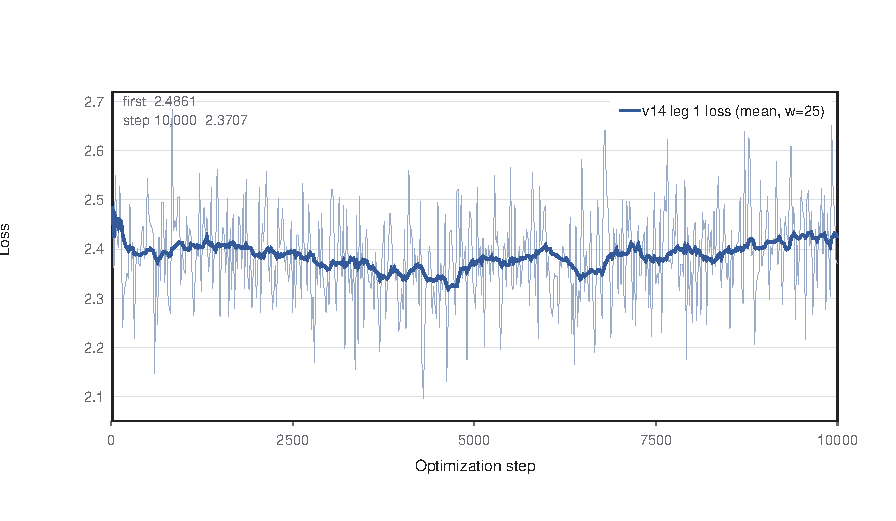
\includegraphics[width=\linewidth]{../figures/fig-loss}
\caption{v14 leg 1 的训练 loss（浅色为逐步记录，深色为 25 步滑动平均）。实测从 2.4861 降到 2.3707。}
\label{fig:fig-loss}
\end{figure}

\begin{center}
\small
\captionof{table}{训练分段}
\begin{tabular}{lrrr}
\toprule
\textbf{段} & \textbf{步区间} & \textbf{状态} & \textbf{说明} \\
\midrule
第一段 & 0 $\rightarrow$ 10,101 & 已完成 & 从 v13 导出续训，\code{chunk\_size} 实际为 64 \\
第二段 & 10,000 $\rightarrow$ 50,000 & \textbf{进行中} & 从 \code{checkpoint-10000} 续训，\code{chunk\_size=128} \\
\bottomrule
\end{tabular}
\end{center}

第一段实测 loss（每 20 步记录）从 \textbf{2.4861} 降到 \textbf{2.3707}； 最后一条 \code{learning\allowbreak{}\_rate = 3\allowbreak{}.6827e\allowbreak{}-05}，与配置的 cosine 在 step 10100 处的 \textbf{理论值 3.68e-05 完全吻合}，说明调度器与进度都正确。

第二段（续训，\code{chunk\_size=128}）在同一区间复现了同样的行为：

\begin{lstlisting}[]
首条  {'loss': 2.4092, 'grad_norm': 2.739, 'learning_rate': 3.681386e-05, 'epoch': 0.15}
末条  {'loss': 2.3686, 'grad_norm': 3.412, 'learning_rate': 3.574538e-05, 'epoch': 0.17}
\end{lstlisting}

LR 从 3.6814e-05 单调降到 3.5745e-05，\textbf{正是 cosine 应当走的轨迹}； loss 在 2.23–2.68 区间波动，与第一段同区间。这同时验证了 \textbf{优化器状态、LR 调度器状态与全局步数都被 HF 正确恢复}。

\begin{notebox}
有一处未解释的观测：第一段在 step 10020 附近的 loss 约 2.47， 第二段同一位置是 2.4092，差约 0.06——远大于 §6.6 实测的 chunk 64/128 单批差异（2.4e-7）。第二段是从 \code{checkpoint-10000} 回滚重跑 （第一段 10001–10101 的 101 步被丢弃），所以两者的数据窗口本应一致。 \textbf{这条我们没有查清}，在 §9 中作为未决项列出。
\end{notebox}

\subsection{一个被踩中过的静默正确性 bug：HF 的损失归一化}

\code{RetNetForCausalLM\allowbreak{}.forward} 签名末尾的 \code{**\_kwargs} 会让 HF 的启发式判定 \code{accepts\allowbreak{}\_loss\allowbreak{}\_kwargs = True}，于是 \code{Trainer\allowbreak{}.training\allowbreak{}\_step} \textbf{跳过}了

\begin{lstlisting}[language=Python]
loss = loss / self.current_gradient_accumulation_steps
\end{lstlisting}

而本模型的损失已按 $\sum w$ 自归一化（并不使用 \code{num\allowbreak{}\_items\allowbreak{}\_in\allowbreak{}\_batch}）。后果是 \textbf{梯度被放大 \code{accum} 倍、等效学习率成倍上升}——静默，且只在 \code{accum > 1} 时发作。 实测症状是 loss 从 3.19 变成 \textbf{12.75 $\approx$ 3.19 $\times$ 4}。修法是在模型类上显式声明：

\begin{lstlisting}[language=Python]
accepts_loss_kwargs = False     # 注意属性名没有 model_ 前缀
\end{lstlisting}

修正后 loss 立刻回到 3.1851 $\rightarrow$ 3.0148，与真实 batch 4 的 3.20 $\rightarrow$ 3.17 一致。

\begin{notebox}
项目此前所有任务都是 \code{accum = 1}，所以这个雷一直没踩到。\textbf{一旦启用梯度累积就必须先修。}
\end{notebox}

\reportrule

\section{工程优化 / Engineering Optimizations}

\subsection{测量方法}

所有步时均在 \code{scripts\allowbreak{}/bench\allowbreak{}\_trainer\allowbreak{}.py} 上测量：它\textbf{复刻} \code{run\_task.py} 的完整路径 （同模型构建、同 \code{TrainingArguments}、同数据集对象、同 collator）， 丢弃前 25 步（含 inductor 首次编译），取\textbf{微步中位数的 4 倍}作为优化步时。

三条纪律，都是踩坑换来的：

\begin{enumerate}
  \item \textbf{一切以墙钟为准。} profiler 的\textbf{算子归因会误导}——它把 \code{NativeDropoutBackward0} 记成 25\%，而实测关掉 dropout 只省 3.9\%。
\end{enumerate}
\begin{enumerate}
  \item \textbf{必须注明供电状态。} 同一个配置在电池下整体慢约 40\%； 早期一次「5.9\% 的旋转缓存收益」就是这么测出来的假象。 本文全部数字均为 \code{BatteryStatus=2}（交流电）下测得。
\end{enumerate}
\begin{enumerate}
  \item \textbf{不能只调算法不看显存。} 关梯度检查点在未腾显存时会内存颠簸， 表现为「算法变慢」——实测同一配置从 1437 ms 骤降到 183 ms 完全来自显存。
\end{enumerate}

\subsection{结果}

\begin{center}
\small
\captionof{table}{优化步时对比}
\begin{tabular}{>{\RaggedRight\arraybackslash}p{255.5pt}>{\RaggedRight\arraybackslash}p{51.1pt}>{\RaggedRight\arraybackslash}p{71.3pt}>{\RaggedRight\arraybackslash}p{47.1pt}}
\toprule
\textbf{配置} & \textbf{优化步时} & \textbf{吞吐} & \textbf{相对 A} \\
\midrule
\textbf{A} 参考：逐块循环，chunk 64，batch 4，梯度检查点，无 compile & 2176 ms & 3764 tok/s & 1.00$\times$ \\
\textbf{B} 批量 chunkwise + \code{torch.compile}，batch 4，梯度检查点 & 903 ms & 8814 tok/s & \textbf{2.41$\times$} \\
\textbf{C} = B + batch1$\times$accum4 + 关梯度检查点 + 8-bit AdamW & 713 ms & 11496 tok/s & \textbf{3.05$\times$} \\
\textbf{C′} = C + 闭式扫描 + 衰减表复用（本文） & \textbf{662 ms} & \textbf{12373 tok/s} & \textbf{3.29$\times$} \\
\bottomrule
\end{tabular}
\end{center}

C′ 相对 B 为 \textbf{1.36$\times$}；相对 C 为 \textbf{1.08$\times$}。 三次重复测量：657 / 662 / 663 ms，抖动 < 1\%。

\textbf{每一项的机理}：

\begin{itemize}
  \item \textbf{A $\rightarrow$ B（2.41$\times$）}：把每块 4 次小矩阵乘（$C=64$ 时每层每步 128 次、
\end{itemize}

全模型 9241 次 \code{aten::matmul}）改成三个跨块批量矩阵乘 + 一次小状态扫描， \code{matmul} 调用降到 441 次。

\begin{itemize}
  \item \textbf{B $\rightarrow$ C（1.26$\times$）}：梯度检查点让每步多跑一整遍前向（前向 1 遍 + 重算 1 遍 +
\end{itemize}

反向 1 遍 = 3 遍，不检查点是 2 遍），\textbf{整整 1/3 的步时是重算出来的}。 关掉它需要先腾显存：8-bit AdamW 把优化器状态从 2.18 GiB 压到 0.55 GiB， 再用 \code{batch 1 × accum 4} 把激活值降到 1/4。

\begin{itemize}
  \item \textbf{C $\rightarrow$ C′（1.08$\times$）}：见 §3.4。
\end{itemize}

\subsection{内核级归因}

\begin{figure}[htbp]
\centering
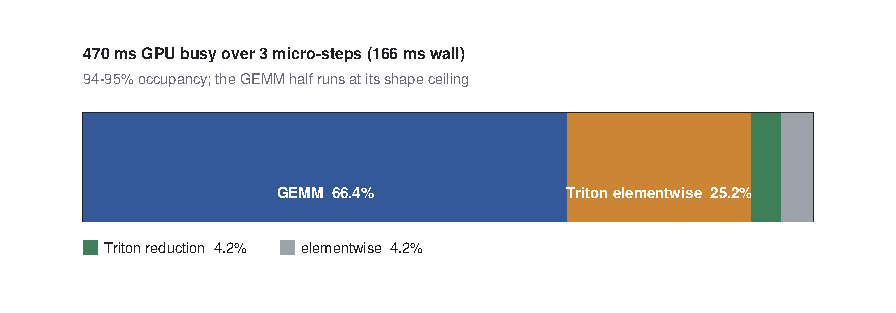
\includegraphics[width=\linewidth]{../figures/fig-kernels}
\caption{C$'$ 下三个微步的 GPU 忙时按 CUDA 内核类别聚合。}
\label{fig:fig-kernels}
\end{figure}

\code{scripts\allowbreak{}/profile\allowbreak{}\_kernels\allowbreak{}.py} 导出 chrome trace 后\textbf{按 CUDA 内核}（而不是算子） 聚合，$C'$ 下 3 个微步的采样：

\begin{center}
\small
\captionof{table}{C$'$ 下按 CUDA 内核聚合的忙时}
\begin{tabular}{lrrrr}
\toprule
\textbf{类别} & \textbf{忙时} & \textbf{占比} & \textbf{内核数} & \textbf{平均} \\
\midrule
GEMM & 312 ms & \textbf{66.4\%} & 2169 & 143.8 $\mu$s \\
Triton 逐元素 & 118 ms & 25.2\% & 3462 & 34.1 $\mu$s \\
Triton 归约 & 20 ms & 4.2\% & 555 & 35.6 $\mu$s \\
\code{elementwise} & 20 ms & 4.2\% & 762 & 25.7 $\mu$s \\
\bottomrule
\end{tabular}
\end{center}

\textbf{总忙时 470 ms / 3 微步 = 157 ms，对墙钟 166 ms = 94–95\% 占用。}

\begin{notebox}
\textbf{一条被推翻的旧结论。} 项目此前用「GPU 忙时 / 墙钟」判定配置 C 有 \textbf{20.8\% 空闲}，据此推断「摘内核没用」。那个数是在\textbf{电池}下测的。 交流电下真实占用是 \textbf{94\%}——前提不成立，「摘内核无用」的结论随之作废。 事实上本文的两处优化（§3.4、§6.4）都是"摘内核"，合计拿回 8\%。
\end{notebox}

\subsection{衰减表的发射次数优化}

\code{\_decay\_tables} 每层构建块内掩码与三张一维衰减表。它只处理 26 万个元素， 却要花 \textbf{410 $\mu$s}——成本几乎全是\textbf{发射延迟}：约 22 个相互依赖的小内核， 而 Windows 上单次发射约 18 $\mu$s。

优化目标因此不是"少算"而是"少发射"：

\begin{enumerate}
  \item 索引张量（\code{arange}/\code{sub}/\code{ge}/\code{clamp}）进缓存，省 4 次发射；
\end{enumerate}
\begin{enumerate}
  \item 三张一维表复用同一个 $\gamma^{\,j}$ 表（$[H,C]$）： $\text{cross} = \gamma^{\,j}\cdot\gamma$、 $\text{value} = \text{flip}(\gamma^{\,j})$、 $\text{chunk} = \gamma^{\,j}[-1]\cdot\gamma$，把 3 次 \code{exp} 压成 1 次。
\end{enumerate}

\textbf{效果}：原本占据 Top-18 的那个 469 $\mu$s 归约核 （\code{triton\allowbreak{}\_red\allowbreak{}\_fused\allowbreak{}\_\allowbreak{}\_to\allowbreak{}\_copy\allowbreak{}\_add\allowbreak{}\_exp\allowbreak{}\_log\allowbreak{}\_mul\allowbreak{}\_select\allowbreak{}\_sum\allowbreak{}\_view\allowbreak{}\_zeros}）\textbf{从榜单消失}， Triton 归约类忙时 \textbf{47 $\rightarrow$ 20 ms}。

\subsection{修复 \code{torch.compile} 的两个静默失效}

项目在 2026-10-10 之前，\code{torch.compile} \textbf{完全无效}，实测 0.0\%。两个独立原因：

\begin{enumerate}
  \item \textbf{没有 Triton。} 笔记本 conda 环境缺 \code{triton-windows}。而 inductor 是\textbf{惰性} 编译，\code{TritonMissing} 要到第一次前向才抛，那时早已离开 \code{train.py} 的 \code{try} 块——所以它\textbf{不崩、不提速、静默地什么都不做}。
\end{enumerate}
\begin{enumerate}
  \item \textbf{编译后的模型从未被调用。} \code{Trainer\allowbreak{}.\allowbreak{}\_\allowbreak{}\_init\allowbreak{}\_\allowbreak{}\_} 把\textbf{原始}模型存进 \code{self\allowbreak{}.model\allowbreak{}\_wrapped}，而 \code{train()} 取的是 \code{self\allowbreak{}.\allowbreak{}\_wrap\allowbreak{}\_model(self\allowbreak{}.model\allowbreak{}\_wrapped)}。 只替换 \code{trainer.model} 的话，编译后的模型永远不会被调用： 日志印着 \code{torch\allowbreak{}.compile applied}、dynamo counters 却是空的、速度毫无变化 （甚至还因 \code{OptimizedModule} 的属性转发慢 1.8$\times$）。
\end{enumerate}

修好后 dynamo counters 显示 \code{\allowbreak{}\textbackslash{}{'frames': \allowbreak{}\textbackslash{}{'total': 1, 'ok': 1\allowbreak{}\textbackslash{}}, 'unique\allowbreak{}\_graphs': 1\allowbreak{}\textbackslash{}}} ——\textbf{一整张图被完整捕获}。

\begin{notebox}
⚠️ 但正是这个"同时替换两个属性"的修法引入了 §7.1 那个更严重的前缀缺陷。 最终解法见 §7.1：\textbf{就地替换 \code{forward}}，而不是包装模块。
\end{notebox}

\subsection{三个死配置字段}

\textbf{\code{config.chunk\_size} 一直是死字段。} \code{RetNetForCausalLM\allowbreak{}.forward} 的签名里 \code{chunk\_size=64} 是\textbf{函数默认值}，而 HF Trainer 调模型时\textbf{不会}传这个关键字， \code{forward} 也\textbf{从不读} \code{self\allowbreak{}.config\allowbreak{}.chunk\allowbreak{}\_size}（它只 \code{getattr(self\allowbreak{}.config,"mode")}）。 实测：

\begin{lstlisting}[]
config.chunk_size = 64 / 128 / 256  ->  loss 全部 2.69759822   （逐位相同 = 配置被忽略）
显式传参 chunk_size = 128           ->  loss 2.69759798        （参数本身有效）
\end{lstlisting}

\textbf{所以项目一直跑在 chunk 64，而任务 JSON、日志、文档全写 128。} \code{bench\_step.py} 的 \code{\allowbreak{}-\allowbreak{}-sweep chunk\allowbreak{}\_size=32,64,128,256} 扫的是空变量， \code{docs/15} §6 那句「chunk 512/1024 反而更慢、最优是 128」\textbf{不成立}。

修复后\textbf{第一次有效的 chunk 扫描}：

\begin{center}
\small
\captionof{table}{chunk 大小扫描}
\begin{tabular}{lrr}
\toprule
\textbf{chunk} & \textbf{优化步时} & \textbf{reserved} \\
\midrule
64 & 663 ms & 6.73 GiB \\
\textbf{128} & \textbf{662 ms} & \textbf{6.61 GiB} \\
256 & 685 ms & 6.90 GiB \\
\bottomrule
\end{tabular}
\end{center}

\textbf{64 与 128 打平，256 慢 3.5\%}——chunk 不是性能杠杆，是管道正确性问题。

\textbf{\code{eval\_batch\_mult} 也是死字段}：\code{run\_task.py} 的配置模板里有它，却从没传给训练脚本， \code{train.py} 里硬编码 \code{*4}。实测 \code{1×4} 时第一次评测要多花 \textbf{128 s} （评测形状重编译），峰值 reserved 冲到 \textbf{7.65 / 8.00 GiB}（离墙只剩 0.35 GiB）； 改成 \code{1×1} 后评测开销从占整轮 \textbf{6.6\% 降到 2.9\%}，reserved 回到 6.73 GiB。

\begin{notebox}
\textbf{实测补充（笔记本上的长跑，按 \code{eval\_runtime} 逐次读）}： 第一段用 \code{per\allowbreak{}\_device\allowbreak{}\_eval\allowbreak{}\_batch\allowbreak{}\_size = 4}，冷启动 276.3 s、\textbf{稳态 57.3 s}； 第二段用 \code{= 1}，冷启动 95.5 s、\textbf{稳态 44.2 s}。 \textbf{稳态对稳态，\code{×1} 比 \code{×4} 快 23\%}，方向与上面的结论一致。

但上面的 \textbf{6.6\%} 是\textbf{冷启动}口径（微基准只测了第一次评测）。 换算成整轮摊销：一轮 2500 步 $\times$ 788 ms = 1970 s， \code{×4} = 57.3/1970 = \textbf{2.9\%}，\code{×1} = 44.2/1970 = \textbf{2.2\%}。 也就是说这个改动的\textbf{方向}有实测支持，\textbf{幅度}比原文说的小（2.9\% $\rightarrow$ 2.2\%，不是 6.6\% $\rightarrow$ 2.9\%）。
\end{notebox}

\textbf{\code{save\_total\_limit} 也是死字段，而且这个会静默删数据。} \code{tasks\allowbreak{}/v14\allowbreak{}\_272m\allowbreak{}\_2k\allowbreak{}\_cont\allowbreak{}.json} 与 \code{tasks\allowbreak{}/v14\allowbreak{}\_272m\allowbreak{}\_2k\allowbreak{}\_resume\allowbreak{}.json} 都写 \code{save\allowbreak{}\_total\allowbreak{}\_limit: 4}， \code{run\_task.py} 的配置模板里有这个键却\textbf{从不拼进命令行}，\code{train.py} 硬编码 \code{save\allowbreak{}\_total\allowbreak{}\_limit=3}。 从落盘的 \code{checkpoint\allowbreak{}-12500\allowbreak{}/training\allowbreak{}\_args\allowbreak{}.bin} 读出实际生效值是 \textbf{3}，四份配置里的 4 一次都没生效。

后果是 \code{checkpoint-10000} 被删掉了。这条链有三段，每段都能独立验证：

\begin{enumerate}
  \item HF 的 \code{\allowbreak{}\_rotate\allowbreak{}\_checkpoints(use\allowbreak{}\_mtime=True, output\allowbreak{}\_dir=run\allowbreak{}\_dir)} （\code{transformers\allowbreak{}/trainer\allowbreak{}.py}，v4.57.6）轮转时\textbf{按目录 mtime 排序而不是按步号}， 超出上限就从最旧的开始 \code{shutil.rmtree}。
\end{enumerate}
\begin{enumerate}
  \item 本文作者在 20:14 用 \code{strip\allowbreak{}\_compile\allowbreak{}\_prefix\allowbreak{}.py \allowbreak{}-\allowbreak{}-in\allowbreak{}-place} 修检查点时， \code{Get-ChildItem} 按名字升序枚举，改写顺序成了 \code{10000 → 5000 → 7500}； \textbf{\code{checkpoint-10000} 因此变成三个里 mtime 最旧的} （落盘时间戳：\code{checkpoint-5000} 20:14:08、\code{checkpoint-7500} 20:14:09，\code{10000} 更早）。
\end{enumerate}
\begin{enumerate}
  \item 20:59 写入 \code{checkpoint-12500} 后目录数是 4 > 3，HF 删掉排序最前的一个——正是它。
\end{enumerate}

\textbf{这一删除是完全静默的}：\code{transformers} 默认日志级别是 \code{WARNING} （实测 \code{transformers\allowbreak{}.utils\allowbreak{}.logging\allowbreak{}.get\allowbreak{}\_verbosity() == 30}），而删除那一行是 \code{logger\allowbreak{}.info("Deleting older checkpoint [\allowbreak{}.\allowbreak{}.\allowbreak{}.] due to args\allowbreak{}.save\allowbreak{}\_total\allowbreak{}\_limit")}， 级别不够，日志里一个字都不会有。\code{logs\allowbreak{}/v14\allowbreak{}\_272m\allowbreak{}\_resume\allowbreak{}.log} 里确实没有。

这也解释了为什么 \code{retnet\_272m\_v13} 和 \code{retnet\_272m\_v14} 都\textbf{只留 3 个}检查点。

\textbf{三个死字段是同一个形状}：配置 JSON 里有 $\rightarrow$ \code{run\_task.py} 不传 $\rightarrow$ \code{train.py} 有默认值。 判据只有一个，而且很便宜：\textbf{读落盘的 \code{training\_args.bin}}，别看配置 JSON。 下面这几个值就是那么读出来的：

\begin{lstlisting}[]
save_total_limit = 3            # 配置 JSON 写 4
logging_steps    = 20           # 于是 log_history 每 20 步一条
save_steps       = 2500
eval_batch_mult  = <absent>     # 不在 TrainingArguments 里，曾是死字段
\end{lstlisting}

\code{logging\_steps=20} 顺手关掉了一个此前存疑的观测：\code{checkpoint-10000} 的 \code{trainer\allowbreak{}\_state\allowbreak{}.json} 里 \code{log\_history} 长 504，一度被怀疑异常；实测 $10000/20 + 4 = 504$（每 2500 步一次共 4 次评测），\code{checkpoint-12500} 是 $12500/20 + 5 = 630$，与实测的 630 逐位吻合——\textbf{它一直就是对的}。

\textbf{已接线}：\code{run\_task.py} 现在把 \code{save\_total\_limit} / \code{save\_steps} / \code{eval\_steps} / \code{weight\_decay} / \code{max\_grad\_norm} 一并拼进命令行，\code{train.py} 对应加了参数 （默认值与原来的硬编码相同，因此只有配置确实不同时行为才变）。 验证方式是 \code{run\allowbreak{}\_task\allowbreak{}.py \allowbreak{}-\allowbreak{}-config \allowbreak{}.\allowbreak{}.\allowbreak{}. \allowbreak{}-\allowbreak{}-dry} 打印出的命令行里出现了 \code{\allowbreak{}-\allowbreak{}-save\allowbreak{}\_total\allowbreak{}\_limit 4}，以及 AST 核对 \code{train.py} 里每个 \code{args.*} 都有对应的 \code{add\_argument}。

\textbf{顺带一个同类但没接线的东西}：\code{--eval\_batches 40} 只被 \code{train.py:429} 的 \code{evaluate()}（非 HF 路径）读取，HF \code{Trainer} 路径的评测跑的是整个验证集—— \code{eval\_runtime} 95.5 s 与此一致。这一条本文\textbf{只做了静态核对，没有实测}。

\subsection{GEMM 到底离硬件上限有多远}

\begin{figure}[htbp]
\centering
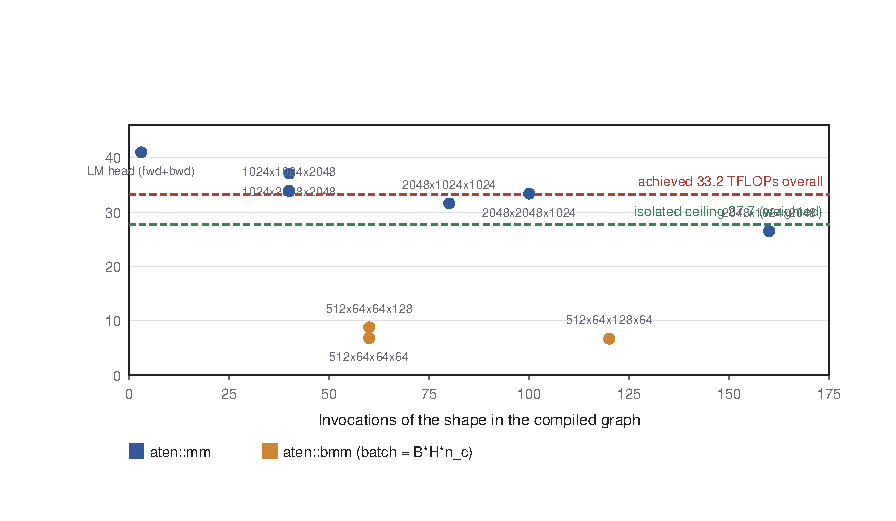
\includegraphics[width=\linewidth]{../figures/fig-gemm}
\caption{编译图实际发出的矩阵乘形状及其现场实测峰值，附两条参考线。}
\label{fig:fig-gemm}
\end{figure}

\textbf{先纠正一个被反复引用的错误数字。} 项目文档写「batch1 形状峰值 11\textasciitilde{}21 TFLOPs」， 实测是 \textbf{26\textasciitilde{}42}（见下表）。拿 batch-4 大方针的 42 TFLOPs 当 batch-1 上限， 会凭空造出「还有 40\% 空间」的假象。

\code{scripts\allowbreak{}/gemm\allowbreak{}\_ceiling\allowbreak{}.py} 用两个实测输入算精确下限： 形状清单直接来自编译图的 dynamo counter \textbf{\code{aten\_mm\_info}}（torch.compile 捕获到的 那张图\textbf{实际发出}的 aten::mm / aten::bmm 调用，计数与 LM head 的 fwd+bwd 三条 各为 1 完全自洽），每个形状的峰值现场测且\textbf{不在调用之间 synchronize} （否则 0.1 ms 级的 chunkwise 批量乘会被 sync 固定开销淹掉，实测低估 3–10 倍）。

\begin{center}
\small
\captionof{table}{编译图实际发出的矩阵乘形状}
\begin{tabular}{lrrrr}
\toprule
\textbf{类型} & \textbf{形状} & \textbf{次数} & \textbf{TFLOPs} & \textbf{小计 ms} \\
\midrule
mm & 2048$\times$1024$\times$2048 & 160 & 26.5 & 51.9 \\
mm & 2048$\times$2048$\times$1024 & 100 & 33.4 & 25.7 \\
mm & 2048$\times$1024$\times$1024 & 80 & 31.6 & 10.9 \\
mm & 1024$\times$2048$\times$2048 & 40 & 37.1 & 9.3 \\
mm & 1024$\times$1024$\times$2048 & 40 & 33.9 & 5.1 \\
mm & LM head 三条 & 各 1 & 40–42 & 6.1 \\
bmm & 512$\times$64$\times$128$\times$64 & 120 & \textbf{6.7} & 9.7 \\
bmm & 512$\times$64$\times$64$\times$64 & 60 & \textbf{6.8} & 2.4 \\
bmm & 512$\times$64$\times$64$\times$128 & 60 & \textbf{8.8} & 3.7 \\
\bottomrule
\end{tabular}
\end{center}

（bmm 的 batch = $B{\cdot}H{\cdot}n_c$；矩阵只有 64$\times$64/64$\times$128，所以只有 6.7–8.8 TFLOPs。）

\textbf{结论：}

\begin{center}
\small
\captionof{table}{实测 GEMM 忙时与形状上限下限}
\begin{tabular}{lr}
\toprule
\textbf{} & \textbf{ms/微步} \\
\midrule
按实测形状峰值的下限 & \textbf{124.6} \\
profiler 实测 GEMM 忙时 & \textbf{104.0} \\
比值 & \textbf{0.83$\times$} \\
\bottomrule
\end{tabular}
\end{center}

\textbf{实测比孤立下限还低。} 换个说法：实际跑到 \textbf{33.2 TFLOPs} （3.457 TFLOP $\div$ 104 ms），而加权形状峰值是 \textbf{27.7 TFLOPs} （3.457 $\div$ 124.6 ms）——\textbf{已经在这批形状的天花板之上}。 两种解释（孤立测量偏保守 / profiler 把部分 matmul 归到了 Triton 桶） 都指向同一结论：\textbf{GEMM 没有可榨的余量。}

剩下的 33.6\% 非 GEMM 是约 3500 个 Triton 逐元素/归约内核，平均 34 $\mu$s、 约 350 GB/s——\textbf{贴着 DRAM 带宽跑}（本机实测拷贝带宽 359–396 GB/s）。 这部分的算术强度只有 0.5–2 FLOP/byte、且与 batch \textbf{无关}， 只能靠融合，而 inductor 已经把可融的都融了。

\subsection{负结果}

\begin{center}
\small
\captionof{table}{chunk 大小扫描}
\begin{tabular}{>{\RaggedRight\arraybackslash}p{104.5pt}>{\RaggedRight\arraybackslash}p{48.3pt}>{\RaggedRight\arraybackslash}p{282.2pt}}
\toprule
\textbf{手段} & \textbf{结果} & \textbf{原因} \\
\midrule
融合线性 + 交叉熵（Liger 式 [12]） & ❌ \textbf{慢 13\%}（batch 1） & 数值等价（loss 逐位相同、梯度相对差 $\leq$2.3e-4）、batch 2 省 452.7 MiB，但分块循环必须 \code{torch\allowbreak{}.\allowbreak{}\_dynamo\allowbreak{}.disable}（否则图断裂卡死），失去编译融合 \\
\code{\allowbreak{}\_head\allowbreak{}\_group\allowbreak{}\_norm} 布局改写 & ❌ \textbf{慢 9.2\%} & 见 §3.5 \\
\code{torch\allowbreak{}.compile(mode="max\allowbreak{}-autotune\allowbreak{}-no\allowbreak{}-cudagraphs")} & ❌ \textbf{0\%}（662 vs 662） & GEMM 走外部 cuBLAS，autotune 只作用于 Triton matmul 模板 \\
CUDA Graphs（\code{mode="reduce\allowbreak{}-overhead"}） & ❌ 不可用 & 与梯度累积硬冲突（同一张图跑 4 次、各自反向） \\
对数深度（Hillis-Steele）扫描 & ❌ \textbf{慢 2.8$\times$} & 每轮 \code{torch.cat} 物化整个 $[B,H,n_c,d_k,d_v]$ \\
物理 batch 2 & ❌ 显存不可行 & 需 9.81 GiB reserved，卡只有 8 GB \\
分层梯度检查点 & ❌ 打不过 C′ & K=10/20 $\rightarrow$ 816 ms \\
\code{dataloader\allowbreak{}\_num\allowbreak{}\_workers} 0/2/4 & ❌ \textbf{0\%} & 数据管线不是瓶颈 \\
去掉损失里的 \code{logits.float()} & ❌ \textbf{0\%} & loss 逐位一致；profile 记的 3.9\% 是归因假象 \\
dropout 0.1 $\rightarrow$ 0.0 & ⚠️ 只省 3.9\% & 且改变正则强度，不划算 \\
\bottomrule
\end{tabular}
\end{center}

\section{正确性缺陷 / Correctness Defects}

本节记录三个\textbf{静默}缺陷。它们的共同点是：\textbf{不报错、不崩溃、日志看起来正常}。

\subsection{\code{\_orig\_mod.} 后缀：所有检查点不可加载}

\code{torch\allowbreak{}.compile(model)} 返回 \code{OptimizedModule}，它把原模型放在 \code{\_orig\_mod} 子模块下， 于是 \code{state\_dict()} 的\textbf{每一个键}都带上 \code{\_orig\_mod.} 前缀。

\code{retnet\allowbreak{}\_hf\allowbreak{}/train\allowbreak{}.py} 为了真正启用编译（§6.5），把编译后的模块同时赋给了 \code{trainer.model} 与 \code{trainer\allowbreak{}.model\allowbreak{}\_wrapped}。HF 的 \code{save\_model} 取的是 \code{self\allowbreak{}.model\allowbreak{}.state\allowbreak{}\_dict()}——\textbf{于是存出来的检查点全带前缀}。

而 \code{RetNetForCausalLM\allowbreak{}.from\allowbreak{}\_pretrained} 加载它们\textbf{不报错}：它把 \code{\_orig\_mod.*} 当作"多余的键"丢掉、把 \code{blocks.*} 当作"缺失的键"\textbf{随机初始化}。结果：

\begin{lstlisting}[]
v13 终版 / rp / v10      365 个键，带前缀 0 个    前向 loss = 2.5767   logits 有限
v14 checkpoint-10000     365 个键，带前缀 365 个  前向 loss = nan      logits 全 nan
\end{lstlisting}

评测侧的表象是 \code{torch.multinomial} 抛 \code{CUDA error: device\allowbreak{}-side assert triggered}——\textbf{从表象根本追不到根因}。

\textbf{回归定位}：v13 的配置 \code{compile=False}，v14 是 \code{compile=True}。 因果链完全闭合。

\textbf{修复（三层）}：

\begin{enumerate}
  \item \textbf{源头}：不再包装模块，改为\textbf{就地替换 \code{forward}}—— \code{trainer\allowbreak{}.model\allowbreak{}.forward = torch\allowbreak{}.compile(trainer\allowbreak{}.model\allowbreak{}.forward)}。 编译照样生效（实测 1.27 it/s，eager 会掉到 0.45），而 \code{state\_dict} 保持干净， 于是\textbf{保存 / 导出 / 续训三条路径同时变正确}。
\end{enumerate}
\begin{enumerate}
  \item \textbf{抢救}：\code{scripts\allowbreak{}/strip\allowbreak{}\_compile\allowbreak{}\_prefix\allowbreak{}.py}，就地剥离前缀并保留 \code{.orig} 备份。
\end{enumerate}
\begin{enumerate}
  \item \textbf{闸门}：\code{verify\_export()} 在每次 \code{save\_model} 后检查键名并响亮报警； \code{scripts\allowbreak{}/check\allowbreak{}\_checkpoints\allowbreak{}.py}（二值、O(1)）与 \code{scripts\allowbreak{}/verify\allowbreak{}\_checkpoint\allowbreak{}\_loads\allowbreak{}.py}（真跑一次前向）供加载前体检。
\end{enumerate}

全部 17 个历史检查点已修复并复核干净，6 个坏备份已删除。

\subsection{续训路径从来没有工作过}

\code{train.py} 原先传 \code{resume\allowbreak{}\_from\allowbreak{}\_checkpoint=args\allowbreak{}.output\allowbreak{}\_dir}。但 HF 的 \code{Trainer\allowbreak{}.\allowbreak{}\_load\allowbreak{}\_from\allowbreak{}\_checkpoint} 是在传入目录里\textbf{直接}找权重文件 （\code{WEIGHTS\_NAME} / \code{SAFE\allowbreak{}\_WEIGHTS\allowbreak{}\_NAME} / …），而 \code{checkpoint-N} 是它的\textbf{子目录}， 所以必然抛：

\begin{lstlisting}[]
ValueError: Can't find a valid checkpoint at checkpoints/retnet_272m_v14
\end{lstlisting}

这条路径此前从未被真正走过（v14 日志里一次 \code{[restart]} 都没有），于是 \code{auto\allowbreak{}\_restart\allowbreak{}\_max: 3} 一直是个\textbf{空承诺}：一旦真的崩了，\code{run\_task.py} 会重启、 立刻再抛同样的错、来回 3 次后退出。现场就是：

\begin{lstlisting}[]
[exit] rc=1
[restart] attempt 1/3 wait 3min
\end{lstlisting}

\textbf{修复}：用 \code{transformers\allowbreak{}.trainer\allowbreak{}\_utils\allowbreak{}.get\allowbreak{}\_last\allowbreak{}\_checkpoint(output\allowbreak{}\_dir)} 解析出 真正的检查点目录再传入，并打印选了哪一个。

\begin{notebox}
这个缺陷还有一个更危险的邻接形态：把检查点修干净之后，resume \textbf{反过来失败}—— HF 以编译模块为目标做 \code{load\_state\_dict}，干净键全被当成"多余键"丢掉。 若不修 §7.1，训练会\textbf{带着 checkpoint 的优化器状态却停在 \code{model\_dir} 的初始权重上}， 而日志只会打印两行 \code{missing\allowbreak{}/unexpected keys} 警告。
\end{notebox}

\subsection{一个"自己跟自己比"的等价性测试}

\code{tests\allowbreak{}/test\allowbreak{}\_fast\allowbreak{}\_chunkwise\allowbreak{}.py} 的设计是：参考实现 vs 批量实现。 但 \code{modeling\allowbreak{}\_retnet\allowbreak{}.\allowbreak{}\_chunkwise\allowbreak{}\_retention} 在环境变量 \code{RETNET\allowbreak{}\_FAST\allowbreak{}\_CHUNKWISE=1} 时 \textbf{直接转发给 \code{chunkwise\_batched}}——而训练环境一直开着这个变量。

\textbf{于是"参考实现"就是被测函数本身}，测试永远报「逐位相同」。 \code{docs/15} §2.3 那张「全部组合 state 逐位相同」的表，\textbf{从未被真正验证过}。

\textbf{修复}：加 \code{reference\_path} 上下文管理器强制按下模块开关； 判据从\textbf{绝对}阈值改成\textbf{相对}量（$\gamma>1$ 的头会把状态放大到 $10^{13}$， 绝对阈值 $10^{-4}$ 毫无意义）。

修复后的真实结论（15 个组合全部通过）：

\begin{center}
\small
\captionof{table}{等价性测试结果}
\begin{tabular}{lrrr}
\toprule
\textbf{gamma} & \textbf{out rel\_mean} & \textbf{out rel\_max} & \textbf{state rel\_max} \\
\midrule
默认初值 0.9688–1.0000 & \textasciitilde{}1.4e-6 & 2.5e-7 – 6.8e-7 & 2.4e-7 – 7.0e-7 \\
\textbf{真实门控 0.6680–1.0117} & \textasciitilde{}8.1e-7 & 9.0e-7 – 2.3e-6 & 5.1e-7 – 2.1e-6 \\
极端 0.30–1.02 & \textasciitilde{}6.2e-7 & 3.1e-7 – 3.6e-6 & 9.3e-7 – 2.7e-6 \\
\bottomrule
\end{tabular}
\end{center}

\textbf{即：快速 chunkwise 路径不是逐位等价，而是相对误差 1e-6 量级的近似} （改动前后同量级，闭式扫描没有让它变差）。

\reportrule

\section{评测 / Evaluation}

\subsection{基准构成}

\begin{figure}[htbp]
\centering
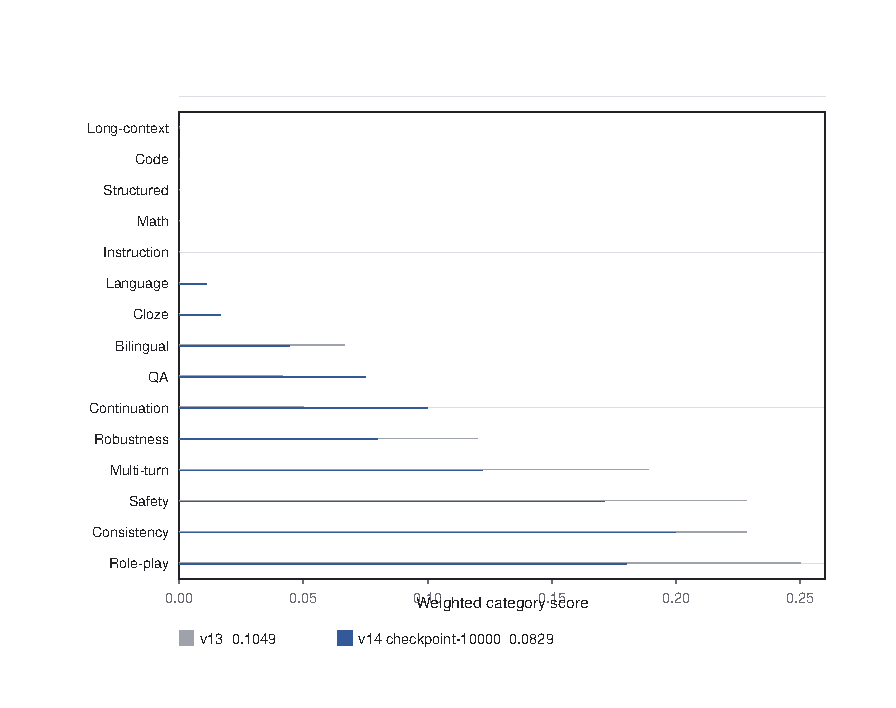
\includegraphics[width=\linewidth]{../figures/fig-bench-cats}
\caption{v13 与 v14 在 15 个类别上的加权得分对照（同一题库、同一种子）。}
\label{fig:fig-bench-cats}
\end{figure}

\code{bench\allowbreak{}/data\allowbreak{}/bench\allowbreak{}\_v3\allowbreak{}.jsonl}：\textbf{1,020 项 / 15 类 / 136 族}， 冻结并带 sha256。解码参数 $T=0.7$、top\_k 40、top\_p 0.9、 repetition\_penalty 1.1、no\_repeat\_ngram 4、单种子 42。

类别分布：角色扮演 100、多轮 90、一致性 70、指令遵循 80、结构化 60、 鲁棒性 50、双语 45、安全 35、填空 120、问答 120、语言 90、续写 60、 长上下文 50、编码 25、数学 25。

\subsection{一个必须写下来的度量缺陷}

\begin{figure}[htbp]
\centering
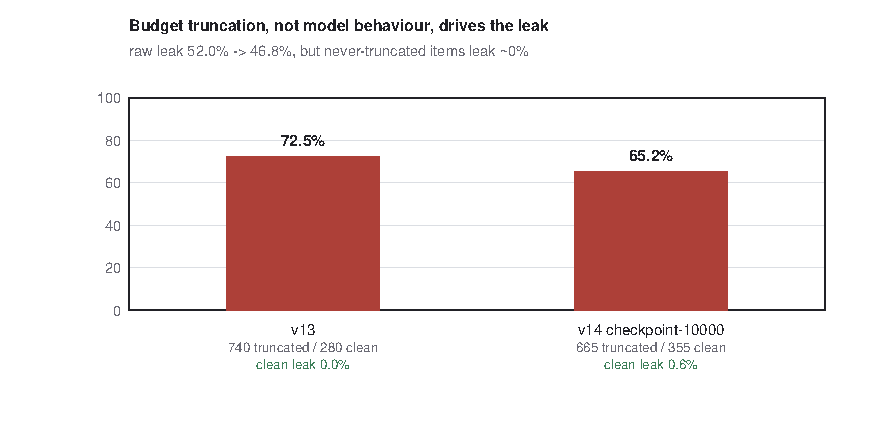
\includegraphics[width=\linewidth]{../figures/fig-truncation}
\caption{按预算截断切分后的截断率；未被截断的项几乎不泄漏。}
\label{fig:fig-truncation}
\end{figure}

\textbf{每道题自带 \code{max\_new}，实测全部落在 16–160（中位 70）}， 而训练数据里 CoT 长度的中位是 \textbf{570 token}（p10 377，p90 1072）。 \textbf{给一个中位要写 570 token 思考的模型 16–160 token 的预算， 它在物理上不可能闭合。}

把主跑结果按「是否被预算截断」切开（判据 $n_{new} = \texttt{max\_new}$， 单轮项是精确的）：

\begin{center}
\small
\captionof{table}{按预算截断切分的泄漏率}
\begin{tabular}{lrrr}
\toprule
\textbf{子集} & \textbf{项数} & \textbf{泄漏率} & \textbf{判据通过} \\
\midrule
单轮 $\cdot$ 被预算截断 & \textbf{644} & \textbf{82.1\%} & 19 \\
单轮 $\cdot$ \textbf{未被截断} & \textbf{235} & \textbf{0.0\%} & 47 \\
多轮（保守下界） & 133 & 0.8\% & 16 \\
\bottomrule
\end{tabular}
\end{center}

\textbf{530 个被判"泄漏"的项全部落在截断子集里；未被截断的 243 项泄漏 0 个。} 裸泄漏率 52.0\% 因此\textbf{不是一个关于模型的数}。

\begin{notebox}
这条结论最初由 \code{docs/17} 提出。我们用\textbf{独立脚本} （\code{scripts\allowbreak{}/audit\allowbreak{}\_leak\allowbreak{}\_truncation\allowbreak{}.py}，只读原始 jsonl、按 id 与题库 join） 复核，\textbf{单轮数字逐位吻合}（644 / 82.1\%、235 / 0.0\%、裸 52.0\%、max\_new 16–160）。

代码侧已修：\code{bench/runner.py} 现在记录 \code{truncated} / \code{max\_new} / \code{think\allowbreak{}\_leak\allowbreak{}\_untruncated}，\code{bench/analysis.py} 输出截断切分 （旧结果文件缺 \code{truncated} 字段时相关项返回 \code{None} 而非 0）； \code{scripts\allowbreak{}/bench\allowbreak{}\_v3\allowbreak{}.py} 增加 \code{--budget} 覆盖开关用于大预算重跑。
\end{notebox}

\subsection{已完成的对照}

\code{rp} / \code{v10} / \code{v13} / \code{v14 checkpoint\allowbreak{}-10000}，同一题库（1,020 项）、同一种子 42、 同一解码参数：

\begin{center}
\small
\captionof{table}{已完成模型的对照}
\begin{tabular}{lrrrrr}
\toprule
\textbf{模型} & \textbf{加权总分} & \textbf{裸泄漏率} & \textbf{被预算截断} & \textbf{未截断项} & \textbf{未截断泄漏} \\
\midrule
\code{v13} & \textbf{0.1049} & 52.0\% & 740（\textbf{72.5\%}） & 280 & \textbf{0.0\%} \\
\code{v14} checkpoint-10000 & \textbf{0.0829} & 46.8\% & 665（\textbf{65.2\%}） & \textbf{355} & 0.6\% \\
\bottomrule
\end{tabular}
\end{center}

\begin{notebox}
截断判据统一用 $n_{new} \ge \texttt{max\_new}\times\text{轮数}$（单轮精确、 多轮是保守下界）；§8.2 表里单轮项的 644 / 82.1\% 是同一判据在单轮子集上的结果。 若改用不含 $\times$轮数 的松规则，v13/v14 的截断率会分别虚高到 76.2\% / 69.1\% ——\textbf{本文不采用那一组数字}，本节以下一律用严格判据。
\end{notebox}

单看这两行会得出「v14 变差了」。但那\textbf{不是}可比的量——两个模型的"未截断子集" \textbf{不是同一批题}（v13 只在更容易收尾的 280 项上停下，v14 停了 355 项）。 必须做\textbf{交集对照}：

\begin{center}
\small
\captionof{table}{交集对照}
\begin{tabular}{lrrrr}
\toprule
\textbf{子集} & \textbf{n} & \textbf{v13} & \textbf{v14} & \textbf{$\Delta$} \\
\midrule
全部 1,020 项 & 1020 & 0.0814 & 0.0716 & $-$0.0098 \\
\textbf{交集：两边都不截断} & \textbf{242} & \textbf{0.1942} & \textbf{0.1405} & \textbf{$-$0.0537} \\
只有 v13 不截断 & 38 & 0.211 & 0.105 & $-$0.106 \\
只有 v14 不截断 & 113 & 0.097 & 0.044 & $-$0.053 \\
两边都截断 & 627 & 0.027 & \textbf{0.048} & \textbf{+0.021} \\
\bottomrule
\end{tabular}
\end{center}

\textbf{结论（含保留）}：

\begin{enumerate}
  \item \textbf{v14 的"停下来"行为确实变好了}——严格判据下截断率 72.5\% $\rightarrow$ 65.2\%， 裸泄漏 52.0\% $\rightarrow$ 46.8\%。这与 \code{docs/17} 关于"开火率才是真缺陷"的判断方向一致。
\end{enumerate}
\begin{enumerate}
  \item \textbf{但在同一批题上，v14 的答题正确率更低}（0.194 $\rightarrow$ 0.141，相对 $-$28\%）， 且四个子集里三个方向一致。
\end{enumerate}
\begin{enumerate}
  \item \textbf{统计功效不足。} 在 242 项上，$p\approx0.17$ 的二项标准误约 0.024， 两个样本的差的标准误约 0.034——$\Delta = -0.054$ 约 \textbf{1.6$\sigma$}。 这\textbf{提示}存在真实退化，但\textbf{不足以定论}。要定论需要多种子（当前只有种子 42）。
\end{enumerate}

\subsection{一个待检验的因果假说：退火后重启学习率}

v14 的配置在\textbf{已经退火到 \code{min\_lr} 的 v13 权重上}重新启动了一条完整的 cosine： 峰值 $4\times10^{-5}$，而 v13 结束时的 LR 是 $1.1\times10^{-5}$——\textbf{跳升 3.6$\times$}。 （当时的理由写在 \code{tasks\allowbreak{}/v14\allowbreak{}\_272m\allowbreak{}\_2k\allowbreak{}\_cont\allowbreak{}.json} 的注释里： 「模型已经退火到 min\_lr，用 $1.1\times10^{-4}$ 重启会先破坏它」， 所以把峰值压到 $4\times10^{-5}$。）

但同时观察到的两个事实是：

\begin{itemize}
  \item v14 的\textbf{训练 loss 更低}（2.4861 $\rightarrow$ 2.3686，而 v13 在 step 10100 是 2.3707）；
\end{itemize}
\begin{itemize}
  \item v14 的\textbf{基准正确率更低}（交集上 0.194 $\rightarrow$ 0.141）。
\end{itemize}

「训练 loss 下降、任务正确率下降」是\textbf{过拟合 / 灾难性遗忘}的典型signature， 而"退火后重启 LR"恰好是一个已知的触发因素。

\textbf{这条我们没有验证}，列在 §9 作为下一轮的首要实验： 用同一份数据、同一段步数，但\textbf{不重启 LR}（从 $1.1\times10^{-5}$ 续走）， 看交集正确率是否回到 v13 水平。

\reportrule

\section{局限与未来工作 / Limitations}

\begin{enumerate}
  \item \textbf{容量。} \code{docs/04} 记录的 CoT 能力门槛在 0.5–1B 参数，272M 在线下。 长上下文（跨 1.2K token 取一个事实）与多步算术在 272M 上稳定为 0， 且 v10（0.28 epoch）也是 0——这两条\textbf{不像是训练量问题}。 但反过来，「训练量不足」也排除不掉：本模型\textbf{从未}把 552M token 的数据看完过一遍 （v13 是 18.5\%，v14 到 50,000 步累计约 92.6\%）。两个方向目前都没有判决性证据。
\end{enumerate}
\begin{enumerate}
  \item \textbf{显存。} 物理 batch 2 需 9.81 GiB reserved，8 GB 卡装不下； 激活值占峰值显存的 59\%，是唯一可动的部分。 \textbf{8 GB 限制的是吞吐，不是容量}——按 \code{docs/16} 的推算（\textbf{未独立核实}， 见引用可靠性说明），打开梯度检查点后同一块卡能装约 700M 参数， 代价是每步 3.3$\times$。
\end{enumerate}
\begin{enumerate}
  \item \textbf{训练/推理不一致。} 训练走 chunkwise、\code{generate()} 预填走 parallel， 两者数值上并不相同，且目前\textbf{没有护栏}。
\end{enumerate}
\begin{enumerate}
  \item \textbf{未验证的引用。} 见参考文献中的标注。
\end{enumerate}
\begin{enumerate}
  \item \textbf{一个未决的能力回归。} v14 在截断校正后的交集上比 v13 低 28\% （0.194 $\rightarrow$ 0.141，约 1.6$\sigma$）。当前只有单种子，\textbf{统计功效不足以下定论}， 但方向一致，且伴随"训练 loss 下降、任务正确率下降"的典型 signature。 首要待检验假说是 §8.4 的\textbf{退火后重启学习率}。
\end{enumerate}
\begin{enumerate}
  \item \textbf{一个未解释的观测。} v13 在 step 10020 附近 loss $\approx$ 2.47， v14 同一位置 2.4092，差约 0.06——远大于实测的 chunk 64/128 单批差异（2.4e-7）。 两者本应看到同一数据窗口（v14 是从 \code{checkpoint-10000} 回滚重跑）。 \textbf{我们没有查清}；候选解释包括数据加载器的跳过语义、 以及第一段那次非正常终止对 RNG 状态的影响。
\end{enumerate}

\section{结论 / Conclusion}

在单张 8 GB 消费级显卡上，RetNet-272M 的优化步时从 \textbf{2176 ms 降到 662 ms（3.29$\times$）}， 全部结论建立在真实 \code{Trainer} 路径的墙钟测量与数值等价性测试之上。 本文的主要算法贡献是一个\textbf{闭式状态扫描}：利用块级衰减在循环内为常量这一事实， 把 $n_c$ 步串行递推替换为一次批量矩阵乘，每层从 1127 $\mu$s 降到 190 $\mu$s， 且相对误差仍在 fp32 累加噪声量级。

更重要的是三条方法论结论：

\begin{enumerate}
  \item \textbf{"已经到极限了"这个判断必须能追溯到测量条件。} 项目曾用电池供电下测得的「20.8\% GPU 空闲」推断"摘内核无用"， 而交流电下真实占用是 94\%——两处真实优化（合计 8\%）恰恰都是"摘内核"。
\end{enumerate}
\begin{enumerate}
  \item \textbf{瓶颈的形态会变。} 优化前是"发射次数"，优化后是"GEMM 的形状上限"。 同一个模型，同一个硬件，答案完全不同。
\end{enumerate}
\begin{enumerate}
  \item \textbf{静默的正确性缺陷比性能问题更贵。} 本文报告的三个缺陷（检查点不可加载、 续训从未工作、等价性测试自比）都没有报错。它们能存活至今，只是因为 \textbf{没有人真的加载过那些检查点}。
\end{enumerate}

\backmattersection{参考文献}\label{sec:refs}

\textbf{[1]} Y. Sun, L. Dong, S. Huang, S. Ma, Y. Xia, X. Zhang, J. Li, F. Wei. *Retentive Network: A Successor to Transformer for Large Language Models.* arXiv:2307.08621, 2023.

\textbf{[2]} S. Yang, B. Wang, Y. Shen, R. Panda, Y. Kim. *Gated Linear Attention Transformers with Hardware-Efficient Training.* arXiv:2312.06635, 2023.

\textbf{[3]} A. Katharopoulos, A. Vyas, N. Pappas, F. Fleuret. *Transformers are RNNs: Fast Autoregressive Transformers with Linear Attention.* arXiv:2006.16236, 2020.

\textbf{[4]} A. Gu, T. Dao. *Mamba: Linear-Time Sequence Modeling with Selective State Spaces.* arXiv:2312.00752, 2023.

\textbf{[5]} T. Dao, A. Gu. *Transformers are SSMs: Generalized Models and Efficient Algorithms Through Structured State Space Duality.* arXiv:2405.21060, 2024.

\textbf{[6]} S. Yang, B. Wang, Y. Zhang, Y. Shen, Y. Kim. *Parallelizing Linear Transformers with the Delta Rule over Sequence Length.* arXiv:2406.06484, 2024.

\textbf{[7]} S. Yang, J. Kautz, A. Hatamizadeh. *Gated Delta Networks: Improving Mamba2 with Delta Rule.* arXiv:2412.06464, 2024.

\textbf{[8]} S. De, S. L. Smith, A. Fernando, A. Botev, G. Cristian-Muraru, A. Gu, et al. *Griffin: Mixing Gated Linear Recurrences with Local Attention for Efficient Language Models.* arXiv:2402.19427, 2024.

\textbf{[9]} B. Peng, E. Alcaide, Q. Anthony, A. Albalak, S. Arcadinho, et al. *RWKV: Reinventing RNNs for the Transformer Era.* arXiv:2305.13048, 2023.

\textbf{[10]} T. Dao, D. Y. Fu, S. Ermon, A. Rudra, C. Ré. *FlashAttention: Fast and Memory-Efficient Exact Attention with IO-Awareness.* arXiv:2205.14135, 2022.

\textbf{[11]} T. Dettmers, M. Lewis, S. Shleifer, L. Zettlemoyer. *8-bit Optimizers via Block-wise Quantization.* arXiv:2110.02861, 2021.

\textbf{[12]} P.-L. Hsu, Y. Dai, V. Kothapalli, Q. Song, S. Tang, S. Zhu, et al. *Liger Kernel: Efficient Triton Kernels for LLM Training.* arXiv:2410.10989, 2024.

\textbf{[13]} I. Loshchilov, F. Hutter. *Decoupled Weight Decay Regularization.* arXiv:1711.05101, 2017.

\textbf{[14]} I. Loshchilov, F. Hutter. *SGDR: Stochastic Gradient Descent with Warm Restarts.* arXiv:1608.03983, 2016.

\textbf{[15]} P. Micikevicius, S. Narang, J. Alben, G. Diamos, E. Elsen, et al. *Mixed Precision Training.* arXiv:1710.03740, 2017.

\textbf{[16]} B. Zhang, R. Sennrich. *Root Mean Square Layer Normalization.* arXiv:1910.07467, 2019.

\textbf{[17]} Y. Wu, K. He. *Group Normalization.* arXiv:1803.08494, 2018.

\textbf{[18]} T. Chen, I. Goodfellow, J. Shlens. *Net2Net: Accelerating Learning via Knowledge Transfer.* arXiv:1511.05641, 2015.

\textbf{[19]} C. Chen, Y. Yin, L. Shang, X. Jiang, Y. Qin, F. Wang, et al. *bert2BERT: Towards Reusable Pretrained Language Models.* arXiv:2110.10329, 2021.

\textbf{[20]} J. Hoffmann, S. Borgeaud, A. Mensch, E. Buchatskaya, T. Cai, et al. *Training Compute-Optimal Large Language Models.* arXiv:2203.15556, 2022.

\textbf{[21]} DeepSeek-AI. *DeepSeek-R1: Incentivizing Reasoning Capability in LLMs via Reinforcement Learning.* arXiv:2501.12948, 2025.

\textbf{[22]} W. Merrill, A. Sabharwal. *The Illusion of State in State-Space Models.* arXiv:2404.08819, 2024.

\textbf{[23]} O. Lieber, B. Lenz, H. Bata, G. Cohen, J. Osin, I. Dalmedigos, et al. *Jamba: A Hybrid Transformer-Mamba Language Model.* arXiv:2403.19887, 2024.

\textbf{[24]} P. Tillet, H.-T. Kung, D. Cox. *Triton: An Intermediate Language and Compiler for Tiled Neural Network Computations.* MAPL@PLDI, 2019.

\reportrule

\subsection{引用可靠性说明}

下列条目转引自本项目内部的调研文档，\textbf{我们没有独立核实}，使用前请自行确认：

\begin{itemize}
  \item \code{docs/18} 引用的 \textbf{arXiv:2507.06457}（linear:full attention 比例与 recall 的
\end{itemize}

340M$\times$20B 受控实验）与 \textbf{arXiv:2605.16640}（hybrid vs pure linear 的 CoT 可解性）。 后者的编号形式可疑（2605 对应 2026 年 5 月），应当核对。

\begin{itemize}
  \item \code{docs/18} 关于「四种线性机制在 340M/20B 下下游差异仅 1.6\%」的量化结论。
\end{itemize}
\begin{itemize}
  \item \code{docs/16} 关于「梯度检查点下 8 GB 可装 54 层 $\approx$ 700M 参数」的推算。
\end{itemize}

\textbf{[1]–[24] 中标注了具体结论的条目，其结论均为本项目自行实测}（出处见正文各节）， 文献仅用于标明方法来源。

\reportrule

\startappendix

\section{附录 A：复现命令 / Appendix A: Reproduction}

\begin{lstlisting}[language=PowerShell]
# 1) 步时对比（真实 Trainer 路径，AC 供电）
$env:RETNET_FAST_CHUNKWISE='1'
python scripts\bench_trainer.py --model_dir checkpoints\retnet_272m_rp `
    --data_dir data_cache\chat_pack_v13 --max_steps 70 --batch_size 1 `
    --grad_accum 4 --chunk_size 128 --compile --no_grad_checkpoint `
    --optim adamw_bnb_8bit --warm_skip 25

# 2) chunk 扫描（修复 config.chunk_size 之后才有意义）
#    把 --chunk_size 依次换成 64 / 128 / 256

# 3) 内核级归因（chrome trace → 按 CUDA 内核聚合）
python scripts\profile_kernels.py --batch_size 1 --grad_accum 4 --chunk_size 128 `
    --compile --no_grad_checkpoint --optim adamw_bnb_8bit --steps 10 --active 3

# 4) GEMM 离上限多远
python scripts\gemm_ceiling.py --reps 25

# 5) 等价性回归（必须）
python tests\test_fast_chunkwise.py      # 15 个组合
python tests\test_head_group_norm.py
python tests\test_control.py             # 外部旗标控制，22 项

# 6) 检查点体检
python scripts\check_checkpoints.py --root checkpoints          # 键名，O(1)
python scripts\verify_checkpoint_loads.py --ckpt <dir>          # 真跑一次前向

# 7) 泄漏率 / 截断切分（只读，无需 GPU）
python scripts\audit_leak_truncation.py --run logs\bench_v3\v13.T0.7_s1.jsonl --by-cat

# 8) 评测
python scripts\bench_v3.py --models "m=checkpoints/retnet_272m_v14/checkpoint-10000" `
    --tokenizer data_cache/chat_pack_v13/bpe_tokenizer.json --seeds 42 `
    --out logs\bench_v3 --tag <tag>
# 大预算重跑（判"会不会闭合"必须放大预算，见 §8.2）
#    追加 --budget 1024

# 9) 训练（笔记本，schtasks 脱离 SSH）
schtasks /create /tn RetNet_v14r /tr "cmd /c C:\Users\Ayaka\RetNet\tasks\start_v14_resume.bat" `
    /sc once /st 23:59 /f
schtasks /run /tn RetNet_v14r
# 优雅停止（不要 taskkill）：
python run_task.py --ctrl next-checkpoint
\end{lstlisting}

\reportrule

\section{附录 B：关键代码 / Appendix B: Key Code}

\subsection{B.1 闭式状态扫描（\code{retnet\allowbreak{}\_hf\allowbreak{}/retention\allowbreak{}\_fast\allowbreak{}.py}）}

\begin{lstlisting}[language=Python]
# (2) 闭式扫描：decay = chunk_decay 在循环里是常量，于是
#     S_prev[i] = d^i·state + Σ_{j<i} d^(i-1-j)·U_j
# 这正是对 T[h,i,j] = d_h^(i-1-j)（下三角）的一次批量矩阵乘。
# 多出来的一行 i=nc 恰好是 new_state。所有指数非负 → 无 γ^-j 溢出。
log_d = torch.log(gamma.to(device=dev, dtype=torch.float32)) * float(chunk_size)
idx = torch.arange(nc + 1, device=dev)
expo_t = idx[:, None] - torch.arange(nc, device=dev)[None, :] - 1
valid_t = expo_t >= 0
T = torch.exp(log_d[:, None, None] * expo_t.clamp_min(0).to(torch.float32)[None])
T = torch.where(valid_t[None], T, torch.zeros((), device=dev, dtype=torch.float32))
T = T.to(q.dtype)                                          # [H, nc+1, nc]

U_flat = U.reshape(B, H, nc, kd * vd)
S_all = torch.matmul(T[None], U_flat)                      # [B,H,nc+1,kd*vd]
if has_state:
    t_state = torch.exp(log_d[:, None] * idx.to(torch.float32)[None]).to(q.dtype)
    S_all = S_all + t_state[None, :, :, None] * state.reshape(B, H, 1, kd * vd)

S_prev = S_all[:, :, :nc].reshape(B, H, nc, kd, vd)
new_state = S_all[:, :, nc].reshape(B, H, kd, vd)
\end{lstlisting}

\subsection{B.2 对数空间衰减掩码（\code{retnet\allowbreak{}\_hf\allowbreak{}/retention\allowbreak{}\_fast\allowbreak{}.py}）}

\begin{lstlisting}[language=Python]
causal, expo, relf = _index_tables(chunk_size, device)
g = gamma.to(device=device, dtype=torch.float32)
log_gamma = torch.log(g)

# exp(log γ · delta)：两个方向都正确饱和。绝不能写成 γ^i · γ^-j ——
# 本模型 γ 最小 0.668，0.668^-255 = 1e44 > 3.4e38 → Inf → NaN。
inner_mask = torch.exp(log_gamma[:, None, None] * expo[None])
inner_mask = torch.where(causal, inner_mask,
                         torch.zeros((), device=device, dtype=torch.float32))

pow1d = torch.exp(log_gamma[:, None] * relf[None, :])     # [H,C] = γ^j
cross_decay = pow1d * g[:, None]                          # γ^(j+1)
value_decay = pow1d.flip(-1)                              # γ^(C-1-j)
chunk_decay = pow1d[:, -1] * g                            # γ^C
\end{lstlisting}

\subsection{B.3 就地编译（\code{retnet\allowbreak{}\_hf\allowbreak{}/train\allowbreak{}.py}）}

\begin{lstlisting}[language=Python]
# 就地替换 forward，**不要**把模型包成 OptimizedModule —— 那会给 state_dict
# 的每一个键加 `_orig_mod.` 前缀，让保存的检查点静默变成随机模型。
compiled_fwd = torch.compile(trainer.model.forward, backend="inductor")
trainer.model.forward = compiled_fwd
\end{lstlisting}

\subsection{B.4 导出自检（\code{retnet\allowbreak{}\_hf\allowbreak{}/train\allowbreak{}.py}）}

\begin{lstlisting}[language=Python]
def verify_export(path) -> bool:
    """safetensors 的键里不能有 `_orig_mod.`，否则 from_pretrained 会静默随机初始化。"""
    ...
    bad = [k for k in keys if k.startswith("_orig_mod.")]
    if bad:
        print(f"[verify] ❌ 导出里有 {len(bad)}/{len(keys)} 个键带 _orig_mod. 前缀 —— "
              f"这个检查点用 from_pretrained 加载会**静默变成随机模型**。")
        return False
    print(f"[verify] ✅ 导出键名干净（{len(keys)} 个），可直接 from_pretrained")
\end{lstlisting}

\subsection{B.5 续训路径（\code{retnet\allowbreak{}\_hf\allowbreak{}/train\allowbreak{}.py}）}

\begin{lstlisting}[language=Python]
if args.resume:
    from transformers.trainer_utils import get_last_checkpoint
    last = get_last_checkpoint(args.output_dir)
    if last is None:
        raise SystemExit(f"--resume 但 {args.output_dir} 里找不到 checkpoint-* 子目录。")
    print(f"[resume] 从 {last} 续训（优化器 / LR 调度器状态由 HF 一并恢复）", flush=True)
    resume_arg = last
else:
    resume_arg = False
trainer.train(resume_from_checkpoint=resume_arg)
\end{lstlisting}

\reportrule

\section{附录 C：外部旗标控制（\code{retnet\allowbreak{}\_hf\allowbreak{}/control\allowbreak{}.py}）}

停一个正在跑的训练原本只能 \code{taskkill}，而且\textbf{顺序还必须对} （\code{run\_task.py} 的 \code{if rc != 0 and attempts < auto\allowbreak{}\_restart\allowbreak{}\_max: 重启}—— 直接杀 \code{train.py} 会拿到 rc=1 而被拉起来）。旗标让训练在\textbf{步边界优雅退出}：

\begin{lstlisting}[]
run               继续（默认；也用来清除指令）
stop              当前优化步做完就停，不等检查点
next-checkpoint   下一次写检查点之后停（检查点先落盘再退出）
save              立刻存一次检查点，然后继续
\end{lstlisting}

正确性依据：\code{transformers\allowbreak{}/trainer\allowbreak{}.py} 的 \code{\allowbreak{}\_inner\allowbreak{}\_training\allowbreak{}\_loop} 里， 2755 行 \code{on\_step\_end} 在 2756 行 \code{\allowbreak{}\_maybe\allowbreak{}\_log\allowbreak{}\_save\allowbreak{}\_evaluate}（存检查点 + 评测） \textbf{之前}，而 break 在 2772 行。所以在 \code{on\_step\_end} 置 \code{control\allowbreak{}.should\allowbreak{}\_training\allowbreak{}\_stop} 会\textbf{先存检查点再退出}—— 这正是「下一个检查点后停」能写对的原因。

\code{stop} / \code{next-checkpoint} 是\textbf{粘性}的（执行后不清旗标）， 这样 \code{run\_task.py} 在进程退出后能分辨"被外部要求停"还是"崩了该重启"。

\reportrule

\section{附录 D：本文报告的缺陷清单 / Appendix D: Defect Summary}

\begin{center}
\small
\captionof{table}{本文报告的缺陷清单}
\begin{tabular}{>{\RaggedRight\arraybackslash}p{12.0pt}>{\RaggedRight\arraybackslash}p{90.2pt}>{\RaggedRight\arraybackslash}p{103.8pt}>{\RaggedRight\arraybackslash}p{101.4pt}>{\RaggedRight\arraybackslash}p{107.6pt}}
\toprule
\textbf{\#} & \textbf{缺陷} & \textbf{症状} & \textbf{为何静默} & \textbf{修复} \\
\midrule
1 & \code{\_orig\_mod.} 前缀 & 检查点加载后 loss=nan & \code{from\_pretrained} 把多余键静默丢弃 & 就地编译 forward + 剥离工具 + 导出自检 \\
2 & 续训路径 & \code{Can't find a valid checkpoint} & 路径从未被真正走过 & \code{get\allowbreak{}\_last\allowbreak{}\_checkpoint()} \\
3 & 等价性测试自比 & 永远报"逐位相同" & 环境变量让参考实现转发到被测函数 & \code{reference\_path} 上下文 + 相对判据 \\
4 & HF 损失归一化 & loss 放大 \code{accum} 倍 & 只在 \code{accum > 1} 时发作 & \code{accepts\allowbreak{}\_loss\allowbreak{}\_kwargs = False} \\
5 & \code{config.chunk\_size} & 配置被忽略 & 无任何报错 & \code{forward} 回落到 config \\
6 & \code{eval\_batch\_mult} & 配置被忽略，评测慢 2.4$\times$ & 无任何报错 & 接线到 \code{train.py} \\
7 & \code{torch.compile} 静默失效 & 日志说 applied、速度 0\% & inductor 惰性编译 + 包装错位 & 显式 \code{import triton} + 就地替换 forward \\
8 & \code{save\_total\_limit} & 配置写 4、实际跑 3，\code{checkpoint-10000} 被轮转删除 & 删除日志是 \code{logger.info}，transformers 默认 \code{WARNING} 不打印 & 接线到 \code{train.py}；判据是读 \code{training\_args.bin}，不看配置 JSON \\
\bottomrule
\end{tabular}
\end{center}

\end{document}
